\documentclass[format=sigconf]{acmart}
\usepackage[utf8]{inputenc}
\usepackage{enumitem}
\usepackage{float}
\usepackage[labelfont=bf,textfont=md]{caption}
\usepackage{graphicx}
\usepackage{xcolor}
\usepackage{minted}
\usepackage{hyperref}
\usepackage[parfill]{parskip}
\usepackage[all]{hypcap}
\usemintedstyle[common-lisp]{default}
\newmintinline[code]{text}{}
\bibliographystyle{plainnat}

\hypersetup{
  colorlinks,
  linkcolor={red!50!black},
  citecolor={blue!50!black},
  urlcolor={blue!80!black}
}

\newlist{step}{enumerate}{10}
\setlist[step]{label*=\arabic*.,leftmargin=2em}

\acmConference[ELS'23]{the 15th European Lisp Symposium}{March 21--22 2023}{%
  }
\acmISBN{}
\acmDOI{}
\setcopyright{rightsretained}
\copyrightyear{2023}

\begin{document}

\title{Experience Report: Kandria - A Game in Common Lisp}

\author{Nicolas Hafner}
\affiliation{%
  \institution{Shirakumo.org}
  \city{Zürich}
  \country{Switzerland}
}
\email{shinmera@tymoon.eu}

\begin{abstract}
  
\end{abstract}

\begin{CCSXML}
  
\end{CCSXML}

\keywords{Common Lisp, Games, Video Games, Computer Graphics, Experience Report}

\maketitle

\def\abovecaptionskip{1pt}
\def\listingautorefname{Listing}
\def\figureautorefname{Figure}

\section{Introduction}\label{introduction}
Kandria is a video game in the ``action RPG'' genre that was released worldwide on the \href{https://kandria.com/steam}{Valve Steam} platform for Windows and Linux in January of 2023, receiving very positive reviews. The game was developed using the Trial engine and thus relies almost entirely upon code and libraries written in Common Lisp -- to our knowledge the first commercial game like this to be released.

\begin{figure}[h]
  \begin{centering}
    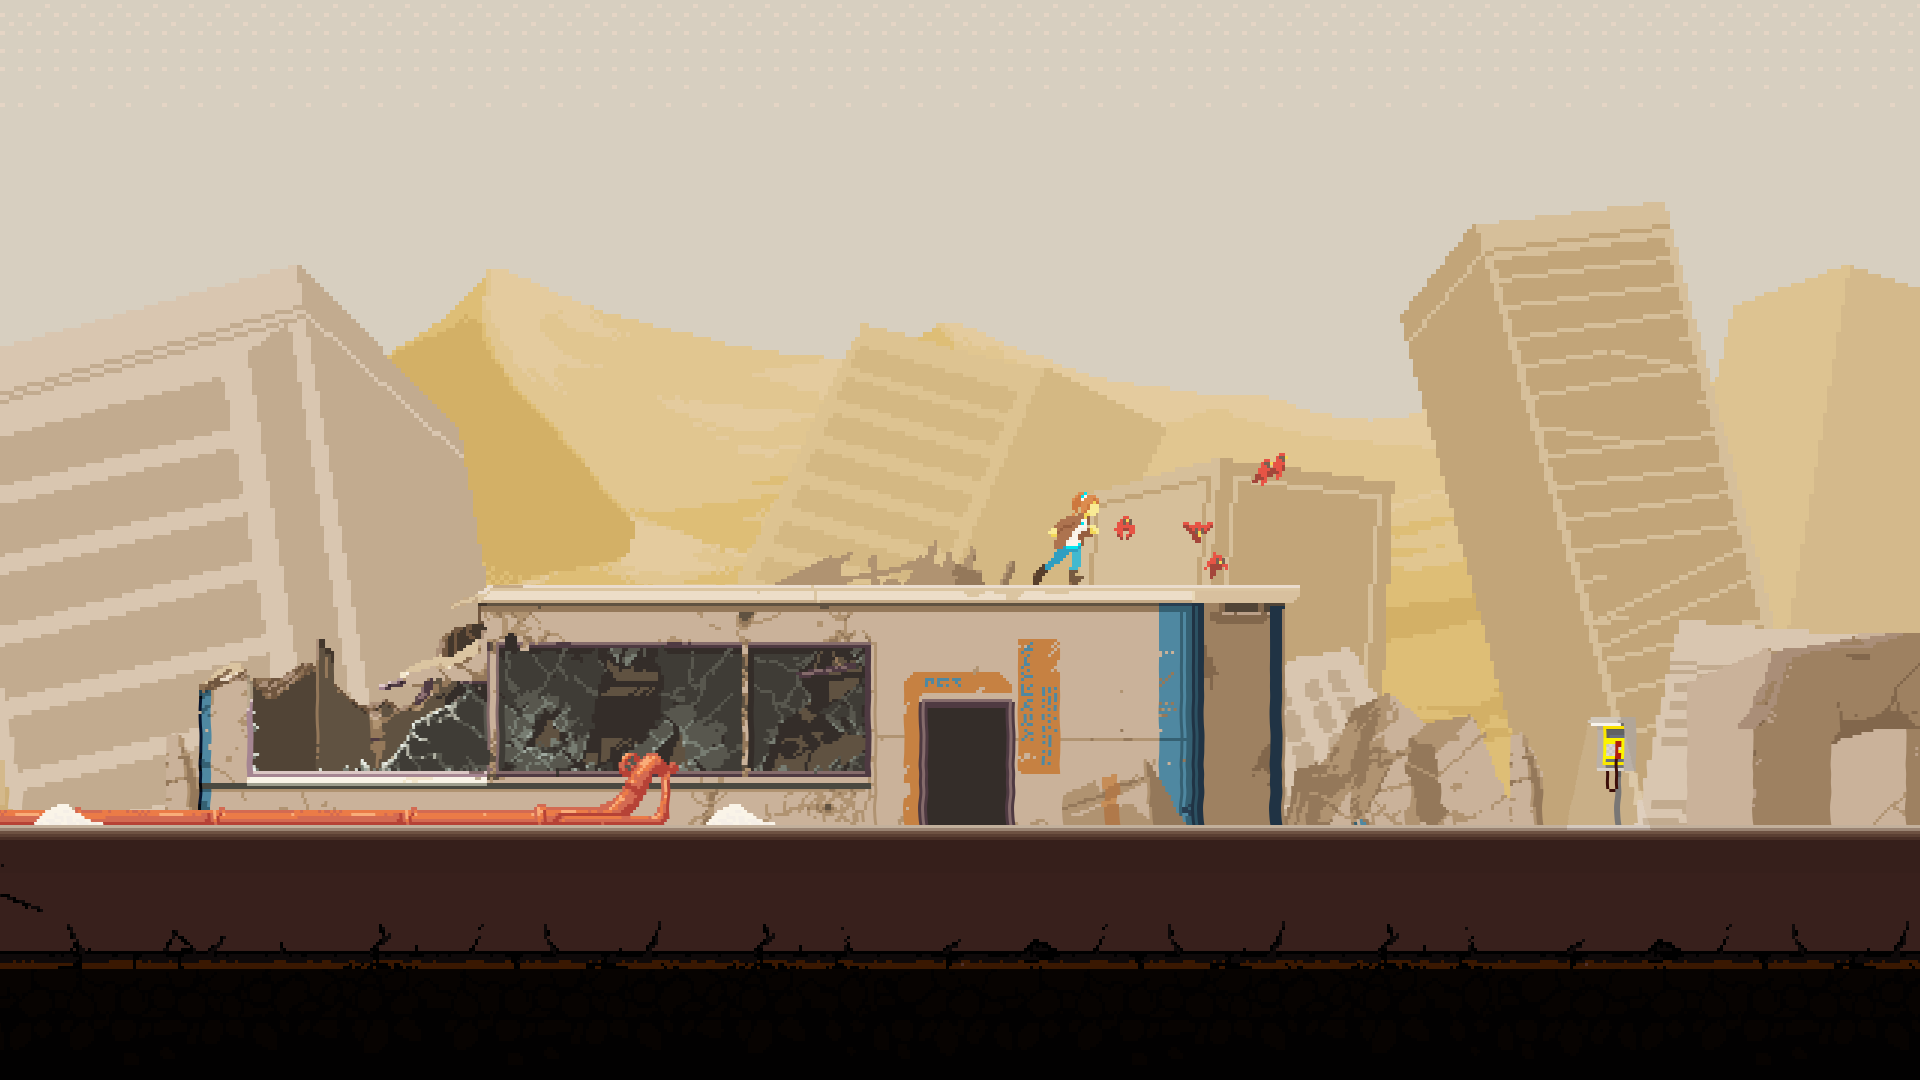
\includegraphics[width=0.4\textwidth]{screenshot 8.png}
  \end{centering}
  \caption{A screenshot of Kandria}
\end{figure}

Games lie at an intersection of many different computer science disciplines such as audio, graphics, interfaces, soft real-time, artificial intelligence, and more. As such games provide a unique challenge in combining all of these disciplines together into one product, and ultimately shipping this product to paying customers.

In this paper we will outline the challenges we faced in realising Kandria as related to Common Lisp, discuss advantages of our approach, and take a look at the work still ahead of us in expanding the capabilities of our engine to better address the requirements of even more complex games we would like to develop in the future.

In particular we will note our own experiences with a few common Boogeymen, such as the overhead of CLOS dispatch, the pause times of GC, the maturity of the library ecosystem, and the stability and size of deployed binaries.

All of our work, including Trial, and even Kandria, is open source and available on our \href{https://github.com/shirakumo}{GitHub}, in the hopes that it will inspire others to create new projects based upon them.

\section{Related Work}\label{relatedwork}
In \cite{hafner2021} we discussed many similar points that this paper touches upon in a format more suitable for people unfamiliar with the intricacies of lisp and especially Common Lisp.

\section{Library Ecosystem}\label{yaks}
In this section we will outline our general experience working in the Common Lisp ecosystem, and particularly the contributions we've made to it in order to implement Kandria.

Out of the 110 libraries Kandria depends upon, 54 were written by us. This does mean that we've spent a rather significant amount of time ``yak shaving'' and creating libraries to fulfil a variety of needs that were, prior to their creation, either completely unfulfilled, or unsatisfactorily so. We will go into detail on some of the more important ones in the following subsections.

While this is undeniably a lot of work, it has been done now and is available to others. Furthermore, of the other half of libraries that we were not authors of, the vast majority have been extremely stable. We only needed to supply extremely minimal patches to a select few libraries, most of which were reviewed and accepted relatively swiftly.

Among this we also count the SBCL implementation itself. While we strive to write implementation independent code in our separate libraries, for Kandria itself we decided to only focus on SBCL in order to reduce the development overhead. SBCL offers great native code performance and is available for all platform configurations that we require. And, perhaps most importantly, it is very actively maintained. Most of the issues we've encountered in releases were usually fixed within a few weeks, if not days.

We are also actively investigating the possibility of porting SBCL and Kandria to the proprietary Nintendo Switch platform, though due to Non-Disclosure Agreements we are unfortunately not at liberty to speak of the specifics involved in that at this time.

We'll now touch on a few specific areas that we developed libraries for. This is by no means exhaustive, but we consider these to be the most relevant to the general community.

\subsection{Math Libraries}\label{math}
While there is no shortage of math libraries available to Common Lisp, especially linear algebra implementations, most of those libraries focus on large scale scientific computing, often by integrating with foreign libraries such as BLAS and LAPACK. For basic computer graphics and especially games, this is overkill. Most of the linear algebra stays within the confines of 2x2, 3x3, 4x4 matrices, and 2, 3, and 4 element vectors.

It is more important to provide a very convenient interface that allows us to perform computations on these elements with adequate speed. Back when Trial started out, no linear algebra libraries with such a limited focus existed, and as such the 3d-Vectors and 3d-Matrices libraries were born. We have since extended this set of libraries to include 3d-Quaternions for common operations with rotations, and 3d-Transforms, for the convenient encapsulation of a ``transform gizmo'' that can represent rotation, translation, and scaling without Gimbal Lock.

All of these libraries rely very heavily on macros to reduce code duplication and automatically generate code for loop unrolling and other common tactics in linear algebra code. The current versions of these libraries all work by emitting an \code{etypecase} for every operation, which then handles dispatch based on the provided argument types. The operation functions are inlined, such that the compiler can eliminate the dispatch altogether if the argument types are locally known. This allows us to provide a generic interface to the user that's quite convenient, while still staying competitive in performance critical sections.

Unfortunately this approach, while portable, is also riddled with issues: since every operation is inlined, this leads to explosive code growth for the compiler before it can reduce the code back down again by eliminating superfluous dispatch \code{etypecase}s. Type inference is also much more complicated, and stack allocation is usually only possible via careful manual rewriting of the operations involved. The libraries are also limited to a single float type, meaning you can by default only create vectors with single-floats as elements.

In this case the lack of static typing facilities and lack of portable compiler hooks for integrating with type inference really hurts the compile speed, implementation clarity, and ultimate performance of the resulting code.

We have started work on a full rewrite of all libraries that take a fundamentally different approach: instead of emitting etypecases and relying on inlining, we create a sort of ``template mechanism'' by which we can generate all possible permutations of a singular function for all involved argument types. This gives us very tiny, but perfectly optimised base functions for all required operations. We then create a dispatcher function on top which falls back to emitting an \code{etypecase} on other implementations, but will hook into SBCL's \code{deftransform} and similar facilities to better handle expansion and type propagation. Finally we create variadic functions on top of the dispatchers which transform any possible variadic call into calls to dispatched 2-argument operation functions, while retaining proper type propagation.

Ultimately this results in much more easily understandable and performing code. However, it still comes at a cost: because we cannot know ahead of time which type combinations and operations the user will actually need, we must generate all possible combinations ahead of time. This potentially results in thousands of functions being generated that are never used. We would like a compiler facility that allows us to hook into the expansion process of a function call to generate the required permutations on-demand.

While such a facility is conceivable, and making it work for unknown runtime types by delayed compilation is, too, we currently have no plans to implement such an advanced strategy. More importantly, we hope that at some point in the future implementors can come to some kind of consensus that would allow a portability library to expose a similar mechanism to SBCL's \code{deftransform} for faster, more convenient, type-inference-informed call expansion.

\subsection{User Interfaces}\label{ui}
When Trial initially began its development in 2016 it was directly integrated with the Qt4 UI toolkit (via CommonQt / Qtools). Since Qt4 is a rather large dependency that not only increases the deployed package size, but also invites a lot of C and C++ interop that can cause hard to debug issues, and has not been maintained in many years, it was quickly abandoned, however. These days Trial does not depend on a UI toolkit directly, or even a specific backend for its OpenGL use.

Aside from CommonQt, the options for a user interface in Common Lisp were, and remain, limited: GTK runs the same issues as Qt, though with even worse deployment and support aspects, LTK is far too limited and cannot integrate with OpenGL at all, McCLIM similarly does not possess an OpenGL backend or method of integration and is still very limited in its theming capabilities, and the newly established CLOG requires a browser to be shipped, which is far too heavy-weight.

As a result we decided to implement our own toolkit, called Alloy. Alloy is separated into different protocols, with the core being completely independent of any rendering or input method, instead only handling the layouting decisions, the input handling via a generic event protocol, and a system to dynamically react to changes in the represented data.

How visual elements can be rendered is then offloaded to several other protocols: the ``Simple Rendering Protocol'' which provides a basic text and shape rendering API, the ``Presentations Protocol'' which allows users to describe how to compose the look of a visual element via the basic shapes from the Simple protocol, and the ``Animations Protocol'' which allows users to describe how shapes change over time as properties of a visual element are changed.

Finally, the Simple protocol needs to be implemented by a backend, such as the ``OpenGL Renderer'' to actually provide a way to draw the shapes in some way, the Core protocol needs to receive input events from the surrounding context to actually react to user input, and some method of rendering and layouting text needs to be provided. Text in particular is separated out as it is a very complex topic in its own right.

This separation of concerns via protocols implemented in CLOS allows us to make Alloy far more amenable to being ported to different backends. In particular, it allows us to use Alloy in contexts that are otherwise rather unusual for UI toolkits, such as within a game where the actual operating system interaction and rendering logic cannot be directly controlled by the toolkit itself, but is instead handled by the game engine.

Usual desktop UI toolkits are rather cumbersome to style effectively, as most desktop applications are expected to present themselves in a ``native look and feel'', while games are expected to have rather elaborately customised and animated interfaces. Alloy's presentations protocol allows us to style the UI quite extensively, with relative ease (\autoref{lst:presentation}).

\begin{listing}
\begin{minted}[fontsize=\small]{common-lisp}
;; Define the shapes that compose the element
(presentations:define-realization (ui alloy:switch)
  ((:border simple:rectangle)
   (alloy:margins)
   :pattern colors:white
   :line-width (alloy:un 2))
  ((:background simple:rectangle)
   (alloy:margins))
  ((:switch simple:rectangle)
   (alloy:extent 0 0 (alloy:pw 0.3) (alloy:ph))))

;; Define how shape properties change
(presentations:define-update (ui alloy:switch)
  (:border
   :hidden-p NIL
   :pattern (if alloy:focus
                (colored:color 0.9 0.9 0.9)
                colors:gray))
  (:background
   :pattern (if (alloy:active-p alloy:renderable)
                colors:dark-accent
                (colored:color 0 0 0 0.5)))
  (:switch
   :pattern (if (alloy:active-p alloy:renderable)
                colors:accent
                colors:black)))

;; Define how to animate the properties
(presentations:define-animated-shapes alloy:switch
  (:background (simple:pattern :duration 0.2))
  (:switch (simple:pattern :duration 0.3)
           (simple:bounds :duration 0.5)))
\end{minted}
\caption{An example of the presentations mechanism in Alloy to define the look and visual behaviour of a switch.}
\label{lst:presentation}
\end{listing}

This protocol separation would not be possible to implement without the high degree of flexibility CLOS offers us in combining behaviours, and even without advanced techniques such as shadow mixins and metaclasses.

\subsection{Input Handling}\label{input}
While keyboard, text, and mouse input is provided by the windowing system on each platform, and thus by whatever OpenGL context backend Trial may use, the same does not go for other input devices, most notably gamepads.

Gamepads or game controllers are special purpose devices composed out of a few analog directional sticks, buttons, and analog pressure triggers. We implemented a library that directly interfaces with the operating system on each of the platforms to discover these devices and read out their state. Thanks to CFFI it is usually unnecessary to actually rely on a C library to interface with operating system APIs, and we can instead write the code directly in Lisp, retaining superior interactive debugging capabilities.

Another challenge, besides the direct system interaction, is that gamepads do not follow a universally defined scheme, and many devices will have partially broken drivers, or simply report their inputs incorrectly. Our library must adapt to this and present as uniform of a scheme to the engine as possible.

To deal with this we have started building a database that maps the device's input IDs onto a standardised set of names and ranges, and have provided a simple setup wizard to configure a new device for which the auto-detection fails.

\subsection{Audio Processing}\label{audio}

\subsection{Operating System Interaction}\label{os}

\subsection{Service Integration}\label{steam}

\section{Garbage Collection}\label{gc}


\section{Performance}\label{performance}


\section{Deployment}\label{deployment}


\section{Conclusion}\label{conclusion}


\section{Further Work}\label{further-work}
Currently a sizable amount of the work in Kandria has not been backported into Trial for more general purpose use. We would like to extract a few of the systems and generalise them to make them available for other users.

We are also working on implementing several new subsystems in Trial to allow creating 3D games, as well. A skeletal animation system has been completed, and we're currently working on a physics subsystem. Also needed will be several spatial query structures to speed up collision testing.

Finally we are also exploring the possibility of porting the engine to work on closed platforms such as the Nintendo Switch. This presents several challenges that we unfortunately cannot elaborate on here due to non-disclosure agreements.

At some point we would like to get rid of the dependency on GLFW to reduce further dependence on C libraries and the issues arising from them. However, GLFW has proven extremely stable in this regard, and as such this is of very low priority for us.

\section{Acknowledgements}\label{acknowledgements}
We would like to thank \textit{you} for being beautiful and nice :)
\bibliography{paper}
\end{document}

%%% Local Variables:
%%% mode: latex
%%% TeX-command-extra-options: "-shell-escape"
%%% TeX-master: t
%%% TeX-engine: luatex
%%% End:
